%
% einschritt.tex -- 
%
% (c) 2015 Prof Dr Andreas Mueller, Hochschule Rapperswil
%
\section{Einschrittverfahren\label{buch:section:ode:einschritt}}
\rhead{Einschrittverfahren}
\index{Einschrittverfahren}%
Die relativ geringe Genauigkeit des Euler-Schrittes beruht darauf,
dass die zu Beginn des Schrittes berechnete Ableitung $f(x_k,y_k)$
nur für das linke Ende des Intervalls $[x_k, x_k+h]$ zutrifft,
weiter rechts im Intervall wird die Abweichung immer grösser.
Eine mögliche Lösung des Problems könnte darin bestehen, statt
nur einer linearen Näherung zusätzliche Glieder der Taylor-Reihe
\begin{equation}
y(x+\Delta x)
=
y(x)
+
y'(x)\cdot \Delta x
+
\frac12 y''(x)\cdot \Delta x^2
+
\frac16 y'''(x)\cdot \Delta x^3
+
o(\Delta x^3)
\label{buch:ode:taylor}
\end{equation}
zu verwenden.
In \eqref{buch:ode:taylor} werden höhere Ableitungen von $y(x)$ benötigt,
während die Differentialgleichung nur die erste Ableitung liefert.
Die höheren Ableitungen wurden aber bereits im
Abschnitt~\ref{grundlagen:hoehere-ableitungen} berechnet.

Wir untersuchen, wie sich das Verfahren für die Beispiel-Gleichung
\eqref{buch:ode:expdgl} anwenden lässt.
Dort gilt
\begin{equation*}
\begin{aligned}
y'(x)&=f(x,y)=-\alpha y
\\
\Rightarrow\qquad
\frac{\partial f}{\partial x}&=0&\frac{\partial f}{\partial y}&=-\alpha.
\end{aligned}
\end{equation*}
Alle zweiten Ableitungen verschwinden.
Die Gleichungen werden damit einfach:
\begin{align*}
y''(x)&=-\alpha f(x,y)=\alpha^2 y
\\
y'''(x)&=\alpha^2f(x,y)=-\alpha^3 y.
\end{align*}
Statt der linearen Approximation sollte daher die kubische Approximation
\begin{equation}
y_{k+1}
=
y_{k}-\alpha h y_k +\frac12\alpha^2 h^2 y_k -\frac16 \alpha^3h^3 y_k
=
y_{k}\underbrace{\biggl(1-\alpha h +\frac12\alpha^2h^2 -\frac16 \alpha^3h^3\biggr)}_{\displaystyle \approx e^{-\alpha h}}
\label{buch:ode:kubisch}
\end{equation}
verwendet werden.
Dass man hier mit einer grösseren Genauigkeit rechnen darf, ist schon daran
erkennbar, dass der Klammerausdruck auf der rechten Seite eine viel
bessere Approximation von $e^{-\alpha x}$ ist also der Faktor
$(1-\alpha h)$ im Euler-Verfahren.
Genauer erwarten wir, dass wir hier ein kubisches Verfahren konstruiert haben.

\begin{table}
\centering
\begin{tabular}{|r|c|r|r|r|}
\hline
$i$&$x$&$e^{-\alpha x}$&Euler&kubisch\\
\hline
 1 & 0.1 & 0.95122942 & 0.\underline{95}000000 & 0.\underline{951229}17 \\
 2 & 0.2 & 0.90483742 & 0.\underline{90}250000 & 0.\underline{904836}93 \\
 3 & 0.3 & 0.86070798 & 0.\underline{85}737500 & 0.\underline{860707}28 \\
 4 & 0.4 & 0.81873075 & 0.\underline{81}450625 & 0.\underline{818729}87 \\
 5 & 0.5 & 0.77880078 & 0.\underline{77}378094 & 0.\underline{778799}73 \\
 6 & 0.6 & 0.74081822 & 0.\underline{73}509189 & 0.\underline{74081}702 \\
 7 & 0.7 & 0.70468809 & 0.\underline{6}9833730 & 0.\underline{70468}675 \\
 8 & 0.8 & 0.67032005 & 0.\underline{6}6342043 & 0.\underline{67031}859 \\
 9 & 0.9 & 0.63762815 & 0.\underline{6}3024941 & 0.\underline{63762}660 \\
10 & 1.0 & 0.60653066 & 0.\underline{5}9873694 & 0.\underline{60652}902 \\
\hline
\end{tabular}
\caption{Näherungswerte für die Lösung $e^{-\alpha x}$ der
Beispieldifferentialgleichung \eqref{buch:ode:expdgl} nach dem Euler-Verfahren
und nach dem kubischen Verfahren \eqref{buch:ode:kubisch} mit einer
Schrittweite von 0.1. Unterstrichen ist jeweils die Stellen, die nach
Rundung auf die angegebene Anzahl stellen mit dem exakten Wert übereinstimmt.
\label{buch:ode:euler-kubisch}}
\end{table}%
In Tabelle~\ref{buch:ode:euler-kubisch} werden die Resultate des
kubischen Verfahrens denen des Euler-Verfahrens gegenübergestellt.
Im ersten Schritt ist der Fehler des Euler-Verfahrens kleiner als $10^{-2}$,
was einer Einheit in der zweiten Nachkommastelle entspricht.
Der Fehler des kubischen Verfahrens ist kleiner als $10^{-6}$, eine
Einheit in der sechsten Nachkommastelle, ungefähr die von einem
kubischen Verfahren zu erwartende Verbesserung.
Nach zehn Rechenschritten liefert das Euler-Verfahren dank Rundung
gerade noch eine korrekte Stelle, während das kubische Verfahren immer noch
gerundet fünf korrekte Stellen gibt.

Es wurde bereits darauf hingewiesen, dass die Terme für die Ableitungen
sehr kompliziert werden.
Noch viel gravierender ist allerdings, dass auch die partiellen Ableitungen
von $f$ nach $x$ und $y$ bekannt sein müssen.
Es ist zwar im Prinzip möglich, diese zu berechnen, der Rechenaufwand 
dafür kann aber so erheblich sein, dass er den Genauigkeitsgewinn
leicht wieder zunichte machen kann.
Praktisch nützliche Verfahren müssen daher danach streben,
die höheren Ableitungen von $y(x)$ ausschliesslich aus Funktionswerten
von $f(x,y)$ zu berechnen.

Wir möchten aber weiterhin nur $y_{k+1}$ ausschliesslich aus $x_k$ und $y_k$
berechnen, also in einem einzelnen Schritt der Form
\[
y_{k+1}=y_k + h\, F(x_k, y_k, h).
\]
Die Funktion $F(x,y,h)$ heisst die {\em Inkrementfunktion}
\index{Inkrementfunktion}%
des Verfahrens.
Für das Euler-Verfahren ist $F(x,y,h)=f(x,y)$.
Es soll also eine Inkrementfunktion gefunden werden, bei der $y(x+\Delta x)$
durch $y(x) + \Delta x\cdot F(x,y,\Delta x)$ bis auf Terme höherer
Ordnung approximiert werden kann.

\subsection{Quadratische Verfahren}
\index{Quadratische Verfahren}%
Ein quadratisches Verfahren verwendet eine Inkrementfunktion $F(x,y,h)$,
welche
\[
y(x+h)=y(x)+hF(x,y,h)+O(h^3)
\]
erfüllt.
Aus den einleitenden Bemerkungen von~\ref{buch:section:ode:einschritt}
folgt, dass dieses Ziel möglicherweise dadurch erreicht werden kann,
dass man Werte von $f$ für verschiedene $x$ geeignet miteinander
kombiniert.
Ein denkbarer Ansatz dafür ist
\[
F(x,y,h)=af(x,y) + bf(x+\alpha h, y +\beta hf(x,y)),
\]
oder anders ausgedrückt: Man führt zuerst etwas Ähnliches wie einen
Euler-Schritt durch, um zum Punkt $(x+\alpha h,y+\beta hf(x,y))$ zu
gelangen.
\index{Euler-Schritt}%
Dort berechnet man den Wert von $f$, und bildet dann einen geeigneten
Mittelwert davon  mit $f(x,y)$.
Durch geeignete Wahl von $a$, $b$, $\alpha$ und $\beta$ sollte es möglich
sein, dass die Inkrementfunktion einen Fehler höchstens dritter Ordnung
hat, womit wir dann ein Integrationsverfahren zweiter Ordnung gewonnen
hätten.

Wir müssen jetzt die Parameter $a$, $b$, $\alpha$ und $\beta$ bestimmen.
Da wir mit dem Übereinstimmen der ersten zwei Ableitungen
nur zwei Bedingungen haben, können wir nicht erwarten, dass wir
eine eindeutige Lösung finden werden.
Vielmehr werden einzelne Parameter frei wählbar sein, es wird eine
ganze Familie von quadratischen Lösungsverfahren entstehen, parametrisiert
durch eine der Variablen $a$, $b$, $\alpha$ und $\beta$.

Wir berechnen nun $F(x,y,h)$ bis zur zweiten Ordnung, damit wird 
$y(x+h)$ bis zur dritten Ordnung ausdrücken können:
\begin{align}
f(x+\alpha h, y + \beta h f(x,y))
&=
f(x,y)+\alpha h\frac{\partial f(x,y)}{\partial x}
+ \beta h \frac{\partial f(x,y)}{\partial y} + O(h^2)
\notag
\\
F(x,y,h)
&=
af(x,y) + bf(x+\alpha h, y + \beta h f(x,y))
\notag
\\
&=
(a+b)f(x,y) + \biggl(\alpha b\frac{\partial f(x,y)}{\partial x}
+ \beta b\frac{\partial f(x,y)}{\partial y} f(x,y))\biggr)h+O(h^2).
\label{buch:ode:inkrementF}
\end{align}
Damit dies bis zur zweiten Ordnung mit dem Inkrement zwischen $x$ und $x+h$
übereinstimmt, muss~\eqref{buch:ode:inkrementF} mit der Taylor-Reihe
von $y(x)$ übereinstimmen, also mit
\begin{equation}
\frac{y(x+h)-y(x)}{h}=y'(x) + \frac12y''(x)h + O(h^2)
=f(x,y) + \frac12\frac{\partial f(x,y)}{\partial x}
+\frac12\frac{\partial f(x,y)}{\partial y}f(x,y) + O(h^2),
\label{buch:ode:ytaylor}
\end{equation}
wobei wir für $y''(x)$ die Gleichung \eqref{grundlagen:2abl} verwendet haben.
Durch Koeffizientenvergleich finden wir die Bedingungen
\[
\begin{aligned}
a+b&=1,&
\alpha b&=\frac12,&
\beta b&=\frac12.
\end{aligned}
\]
Einzig $b$ kommt in allen drei Gleichungen vor, und bestimmt den Wert der
jeweiligen anderen Variablen:
\[
\begin{aligned}
a&=1-b,&\alpha&= \beta=\frac{1}{2b}.
\end{aligned}
\]
Jeder Wert von $b$ zwischen $0$ und $1$ liefert ein Verfahren mit quadratischer
Genauigkeit.

\begin{figure}
\centering
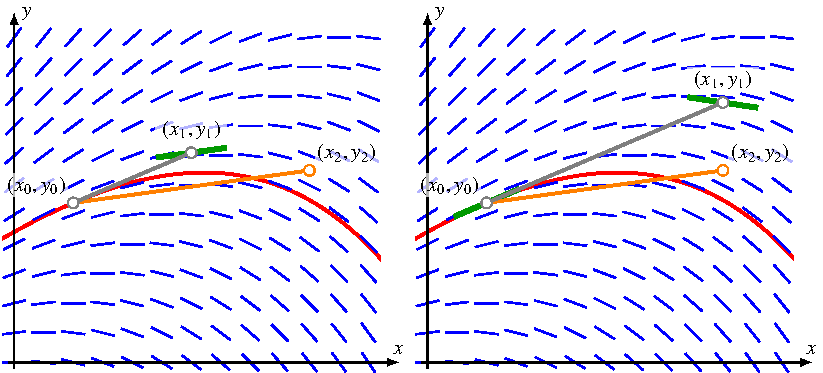
\includegraphics{chapters/50-ode/figures/ordnung2.pdf}
\caption{Einschrittverfahren zweiter Ordnung.
\index{Euler-Verfahren!verbessert}%
\index{verbessertes Euler-Verfahren}%
Das verbesserte Euler-Verfahren (links) führt zunächst einen Euler-Schritt
halber Länge mit der Steigung $f(x_0,y_0)$ (grau) aus und verwendet
die bei $(x_1,y_1)$ gefundene Steigung 
$f(x_1,y_1)$ (grün) für einen ganzen Euler-Schritt (orange),
der zu $(x_2,y_2)$ führt.
\index{Runge-Kutta-Verfahren!vereinfacht}%
\index{vereinfachtes Runge-Kutta-Verfahren}%
Das vereinfachte Runge-Kutta-Verfahren (rechts) führt einen ganzen
Euler-Schritt (grau) aus, der zu $(x_1,y_1)$ führt.
Dann wird der Mittelwert der Steigungen $f(x_0,y_0)$ und $f(x_1,y_1)$
(grün) für einen ganzen Euler-Schritt verwendet, der zu $(x_2,y_2)$ führt
(orange).
\label{buch:einschritt:figure:ordnung2}}
\end{figure}

Der Parameterwert $b=1$ führt auf $\alpha=\beta=1$ und $a=0$, die
Rekursionsformel ist in diesem Falle
\begin{equation}
y_{k+1}=y_{k}+hf\biggl(x_k+\frac{h}2,y_k+\frac{h}2 f(x_k,y_k)\biggr).
\label{buch:ode:improved-euler}
\end{equation}
Das Verfahren führt also erst einen halben Euler-Schritt zum Punkt
$(x_k+\frac12h,y_k+\frac{h}2f(x_k,y_k))$ durch, berechnet dort mit Hilfe
von $f$ die Steigung, die dann für einen Euler-Schritt der Länge $h$
verwendet wird
(Abbildung~\ref{buch:einschritt:figure:ordnung2} links).
Daher heisst dieses Verfahren auch das {\em verbesserte Euler-Verfahren}.
\index{Euler-Verfahren!verbessert}%
\index{verbessertes Euler-Verfahren!verbessertes}%

Verwendet man $b=\frac12$, folgt zunächst $a=\frac12$ und $\alpha=\beta=1$.
Daraus erhält man die Rekursionsformel
\begin{equation}
y_{k+1}=y_k+\frac{h}2\biggl(
f(x_k,y_k) + f(x_k+h, y_k + hf(x_k,y_k))
\biggr).
\label{buch:ode:simplified-runge-kutta}
\end{equation}
In diesem Verfahren
(Abbildung~\ref{buch:einschritt:figure:ordnung2} rechts)
führt man also zuerst einen Euler-Schritt der Länge
$h$ durch, mit dem man zum Punkt $(x_k+h, y_k+hf(x_k,y_k))$ gelangt.
Dort berechnet mit mit Hilfe von $f$ die Steigung.
Das arithmetische Mittel dieser Steigung mit der im Euler-Verfahren
verwendeten Steigung $f(x_k,y_k)$ im Punkt $x_k$ wird dann als
Steigung für einen Euler-Schritt verwendet.
Statt eines einzigen Steigungswertes werden hier also zwei Steigungswerte
von den Enden des Intervalls $[x_k,x_{k+1}]$ gemittelt.
Wegen der Ähnlichkeit dieses Vorgehens mit dem später zu besprechenden
Runge-Kutte-Verfahren heisst diese Verfahren auch das
{\em vereinfachte Runge-Kutta-Verfahren}.
\index{Runge-Kutta-Verfahren!vereinfacht}%
\index{vereinfachtes Runge-Kutta-Verfahren}%

\subsection{Runge-Kutta-Verfahren\label{subsection:buch:ode:runge-kutta}}
\index{Runge-Kutta-Verfahren}%
\begin{figure}
\centering
%\includegraphics{chapters/images/numerik-4.pdf}
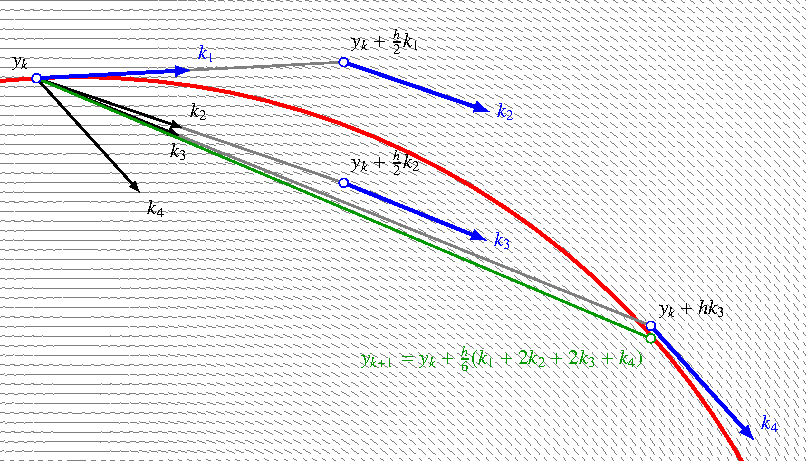
\includegraphics{chapters/50-ode/figures/rungekutta.pdf}
\caption{Zusammenspiel der Richtungen $k_1$ bis $k_4$ bei einem
Einzelschritt des Runge-Kutta-Verfahrens vierter Ordnung.
Der nächste Punkt $y_{k+1}$ wird gemäss
Formel~\eqref{buch:ode:runge-kutta-rekursion} berechnet.
\index{Runge-Kutta-Verfahren}%
\label{buch:ode:rk-step}}
\end{figure}
Das {\em Runge-Kutta-Verfahren} erweitert die Inkrementfunktion derart,
dass der Einzelschritt bis zur fünften Ordnung mit der Taylor-Reihe von
$y(x)$ übereinstimmt.
\index{Taylor-Reihe}%
\index{Runge-Kutta-Verfahren}%
So entsteht ein Verfahren vierter Ordnung, es stellt einen guten Kompromiss
zwischen Genauigkeit und Rechenaufwand dar.
\index{Genauigkeit}%
\index{Rechenaufwand}%

Da vier Ableitungen korrekt dargestellt werden müssen, ist zu erwarten,
dass vier verschiedene Werte von $f$ an verschiedenen Punkten $(x,y)$
ausgewertet und geeignet miteinander kombiniert werden müssen.
Genauer: Man bestimmt zuerst die Werte
\begin{align*}
k_1&=f(x_k,y_k)\\
k_2&=f\biggl(x_k+\frac{h}2,y_k+\frac{h}2k_1\biggr)\\
k_3&=f\biggl(x_k+\frac{h}2,y_k+\frac{h}2k_2\biggr)\\
k_4&=f(x_k+h, y_k+hk_3)
\end{align*}
und setzt diese dann zusammen, um den nächsten Wert $y_{k+1}$
zu berechnen:
\begin{equation}
y_{k+1} = y_k + \frac{h}6(k_1 + 2k_2 + 2k_3 + k_4)
\label{buch:ode:runge-kutta-rekursion}
\end{equation}
(Abbildung~\ref{buch:ode:rk-step}).
Man kann die Formeln wie folgt interpretieren.
\begin{enumerate}
\item
Zuerst wird ein halber Euler-Schritt mit der Steigung $k_1=f(x_k,y_k)$,
durchgeführt, und am Zielpunkt die Steigung $k_2$ ermittelt.
\item
Mit dieser Steigung $k_2$ wird dann erneut ein halber Schritt von $(x_k,y_k)$
aus durchgeführt, und am Zielpunkt erneut die Steigung $k_3$ ermittelt.
\item
Mit $k_3$ führt man einen ganzen Schritt aus, an dessen Zielpunkt man die
Steigung $k_4$ findet.
\item
Diese vier Steigungen werden jetzt gewichtet gemittelt, wobei
$k_2$ und $k_3$ doppeltes Gewicht erhalten, und mit dieser
Steigung wird ein ganzer Schritt vorgenommen.
\end{enumerate}

Die Formeln für die $k_i$ sowie \eqref{buch:ode:runge-kutta-rekursion}
können ganz ähnlich wie das verbesserte Euler-Verfahren bzw.~das
vereinfachte Runge-Kutta-Verfahren begründet werden.
Der Aufwand dafür ist aber beträchtlich, so dass wir auf die
detaillierte Darstellung dieser Herleitung verzichten wollen.

\begin{table}
\centering
\begin{tabular}{|r|c|r|r|r|r|r|}
\hline
$i$& $x$ & $y(x)=e^{-\alpha x}$&Euler&verbessert&vereinfacht&Runge-Kutta\\
\hline
 0 & 0.0 & 1.00000000 & 1.000 & 1.00000000 & 1.00000000 & 1.0000000000 \\
 1 & 0.1 & 0.95122942 & 0.\underline{95}0 & 0.\underline{9512}5000 & 0.\underline{9512}5000 & 0.\underline{95122942}71 \\
 2 & 0.2 & 0.90483742 & 0.\underline{90}2 & 0.\underline{9048}7656 & 0.\underline{9048}7656 & 0.\underline{9048374}229 \\
 3 & 0.3 & 0.86070798 & 0.\underline{85}7 & 0.\underline{8607}6383 & 0.\underline{8607}6383 & 0.\underline{8607079}834 \\
 4 & 0.4 & 0.81873075 & 0.\underline{81}4 & 0.\underline{8188}0159 & 0.\underline{8188}0159 & 0.\underline{8187307}620 \\
 5 & 0.5 & 0.77880078 & 0.\underline{77}3 & 0.\underline{7788}8502 & 0.\underline{7788}8502 & 0.\underline{7788007}936 \\
 6 & 0.6 & 0.74081822 & 0.\underline{73}5 & 0.\underline{7409}1437 & 0.\underline{7409}1437 & 0.\underline{7408182}327 \\
 7 & 0.7 & 0.70468809 & 0.\underline{69}8 & 0.\underline{704}79480 & 0.\underline{704}79480 & 0.\underline{7046881}031 \\
 8 & 0.8 & 0.67032005 & 0.\underline{6}63 & 0.\underline{670}43605 & 0.\underline{670}43605 & 0.\underline{6703200}606 \\
 9 & 0.9 & 0.63762815 & 0.\underline{6}30 & 0.\underline{637}75229 & 0.\underline{637}75229 & 0.\underline{6376281}672 \\
10 & 1.0 & 0.60653066 & 0.\underline{5}98 & 0.\underline{606}66187 & 0.\underline{606}66187 & 0.\underline{6065306}762 \\
\hline
\end{tabular}
\caption{Vergleich der Genauigkeit der verbesserten numerischen Verfahren.
Unterstrichen jeweils die nach Rundung korrekten Stellen der Lösung.
\label{buch:ode:genauigkeit}}
\end{table}


\begin{table}
\centering
\begin{tabular}{|l|l|c|r|>{$}r<{$}|}
\hline
Verfahren                           &$h$  &Schritte&$y_n$&\text{Fehler}\\
\hline
Euler-Verfahren                     &0.025&  40    & 0.\underline{60}462232 &  0.00190834 \\
verbessertes Euler-Verfahren        &0.05 &  20    & 0.\underline{6065}6285 & -0.00003219 \\
vereinfachtes Runge-Kutta-Verfahren &0.05 &  20    & 0.\underline{6065}6285 & -0.00003219 \\
Runge-Kutta-Verfahren               &0.1  &  10    & 0.\underline{6065306}7 & -0.00000001 \\
\hline
\end{tabular}
\caption{Vergleich der verschiedenen Verfahren bei gleichbleibendem 
Rechenaufwand.
\index{Schrittweite}%
Die Schrittweite wurde jeweils so angepasst, dass in allen Verfahren bis
zum Wert $x=1$ die gleiche Anzahl von Auswertungen der Funktion $f$
notwendig wurde.
\label{buch:ode:vergleich-aufwand}}
\end{table}

Die Tabelle~\ref{buch:ode:genauigkeit} demonstriert die überragende
Genauigkeit des Runge-Kutta-Verfahrens.
\index{Genauigkeit}%
Trotz der relativ grossen Schrittweite von $h=0.1$ erreicht das
Verfahren nach zehn Schritten eine Genauigkeit von sieben signifikanten
Stellen.
Da in jedem Schritt die Funktion $f$ viermal ausgewertet werden muss,
ist der Rechenaufwand mit dem Runge-Kutta-Verfahren viermal grösser
als im Euler-Verfahren, letzteres kann aber mit nur einer signifikanten
Stelle kaum als brauchbar bezeichnet werden.
\index{Euler-Verfahren}%
Passt man in jedem Verfahren die Schrittweite so an, dass für die
Berechnung der Näherung für $y(1)$ immer gleich viele Auswertungen
der Funktion $f(x,y)$ nötig sind, ergeben sich die Resultate in
Tabelle~\ref{buch:ode:vergleich-aufwand}.
Bei gleichem Rechenaufwand ist das Runge-Kutta-Verfahren um viele
Grössenordnungen präziser.
Es gibt daher eigentlich keinen praktischen Grund, überhaupt je etwas
anderes als das Runge-Kutta-Verfahren zu verwenden.


